\documentclass[a4paper,12pt]{article}

\usepackage{geometry}       % Required for page layout.
\usepackage{hyperref}       % Required for hyperlinks.
\usepackage{graphicx}       % Required for figures.
\usepackage{subfig}         % Required for minipages.
% \usepackage{caption}
% \usepackage{subcaption}
\usepackage{placeins}
\usepackage{float}

\newgeometry{vmargin={25.4mm}, hmargin={27mm,27mm}}
\setlength\parindent{0pt}   % Disable paragraph indent.

\title{Project 3: Monte Carlo and Molecular Dynamics}
\author{
  Elias Rilegård\\
  \texttt{eliasril@kth.se}
}

\begin{document}
\maketitle

\section*{Exercise 3.1: Monte Carlo}

The task of this exercise was to use the Metropolis method to calculate the following average:

$$
  \left\langle x \right\rangle = \frac{
    \displaystyle \int_{0}^{\infty} x e^{-x} \,\mathrm{d}x
  }{
    \displaystyle \int_{0}^{\infty} e^{-x} \,\mathrm{d}x
  }
$$

By setting $P(x) = e^{-x}$, using $P(x) = 0$ for $x < 0$ (since this method is originally designed for integrals
where the range is $(-\infty, \infty)$, setting this condition effectively limits the integrals to $(0, \infty)$)
and varying $\delta$ between $0.01$ and $10$ (in logarithmic steps), we get the following estimations:

\begin{figure}[!ht]
  \centering
  \begin{minipage}{0.49\textwidth}
    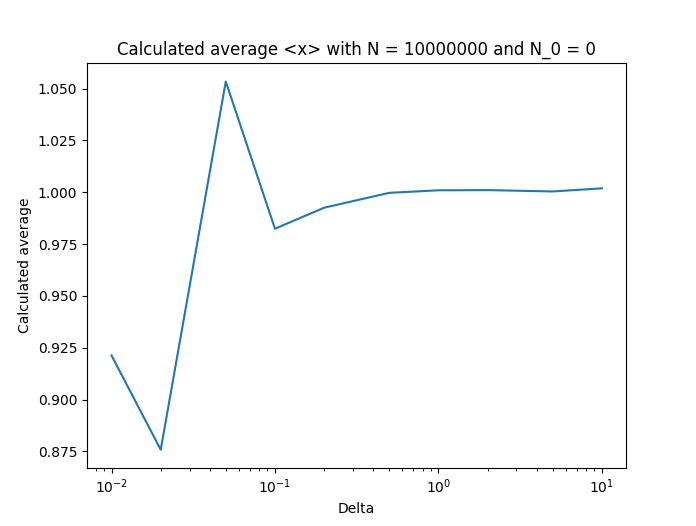
\includegraphics[width=\textwidth]{img/3_1_N0_0.png}
  \end{minipage}
  \begin{minipage}{0.49\textwidth}
    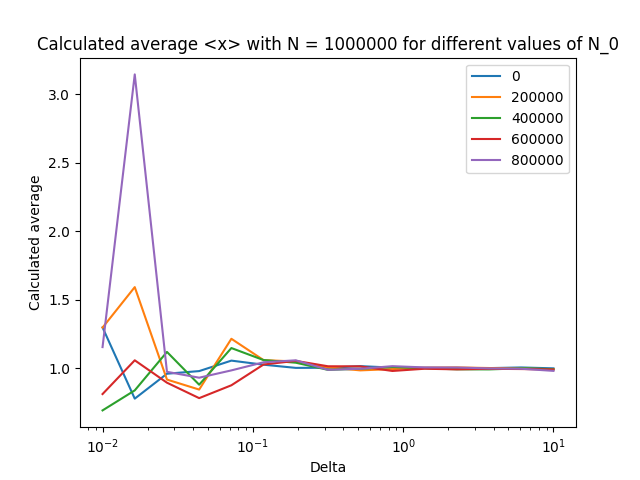
\includegraphics[width=\textwidth]{img/3_1_multiple_N_0.png}
  \end{minipage}
\end{figure}

If we let $x_0 = 0$, the choice of $N_0$ is irrelevant as the estimation converges to the correct value regardless.
However, to be exhaustive, the same estimation has been calculated using different values of $N_0$ from $0$ to $0.8N$,
in steps of $0.2N$. As is clear from the plot, when using $x_0 = 0$, the estimation converges quickly to the correct
value, regardless of $N_0$.

Analytically, this average can be computed to be equal to $1$, so the calculations are correct. However, as is the
case with every simulation, error terms will be present. In this case, the error term looks like $\sigma / \sqrt{N}$,
where $\sigma^2 = \left\langle f^2 \right\rangle - \left\langle f \right\rangle^2$ is the variance, here 
$\left\langle \cdot \right\rangle$ denoting the average. Computing the error term for different values of $N$ yields
the following plot:

\begin{figure}[!ht]
  \centering
  \begin{minipage}{0.49\textwidth}
    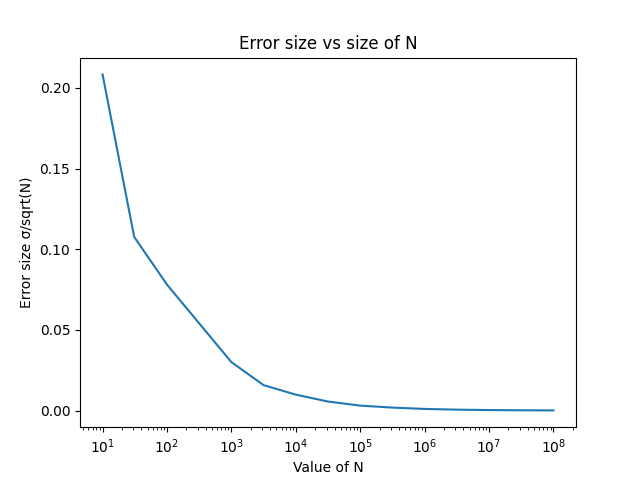
\includegraphics[width=\textwidth]{img/3_1_error_size.png}
  \end{minipage}
  \begin{minipage}{0.49\textwidth}
    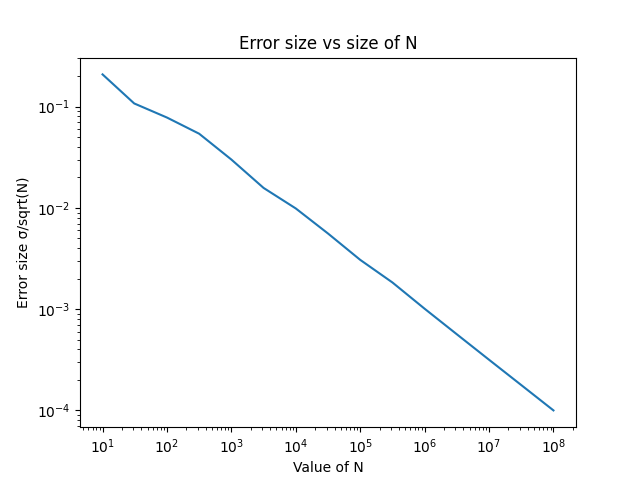
\includegraphics[width=\textwidth]{img/3_1_error_size_loglog.png}
  \end{minipage}
\end{figure}

As $N$ increases, the error term approaches zero, albeit rather slowly, since Monte Carlo-simulations have an order
of convergence of $\frac{1}{2}$. By the time $N$ has reached $10^5$ to $10^6$, the error term is small enough to be
pretty much negligible. 

\section*{Exercise 3.2: Molecular Dynamics}

For this exercise, a template was provided to simulate particles in different conditions.

\subsection*{Part a}

Implementing the Lennard-Jones potential and force as

$$
  V_{ij}(r_{ij}) = 4\epsilon_{ij}\left[ \left( \frac{\sigma_{ij}}{r_{ij}} \right)^{12} - \left( \frac{\sigma_{ij}}{r_{ij}} \right)^6 \right]
  \quad
  \mathbf{F}(\mathbf{x}) = -\nabla V = -\frac{\mathrm{d}V}{\mathrm{d}r}
$$

respectively, then setting $\epsilon_{ij} = \sigma_{ij} = 1$ for simplicity, we arrive at a model which gives good
conservation of the total energy in the system. Using a temperature $T = 1$, we increase the timestep \texttt{dt}
until things go very wrong:

\begin{figure}[!ht]
  \centering
  \begin{minipage}{0.49\textwidth}
    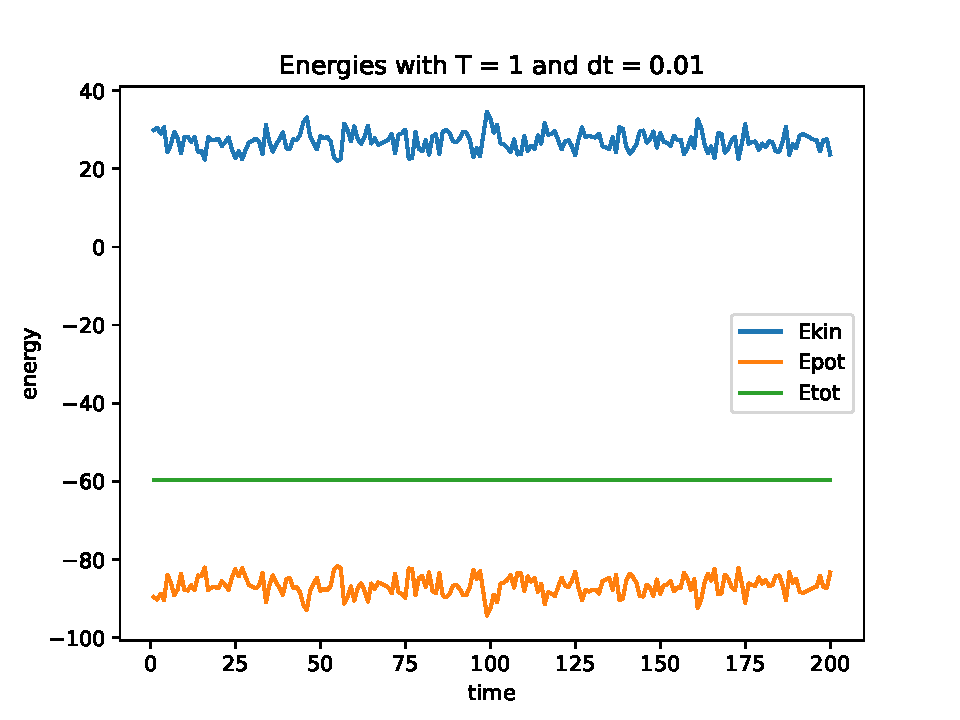
\includegraphics[width=\textwidth]{img/3_2a_dt001.pdf}
  \end{minipage}
  \begin{minipage}{0.49\textwidth}
    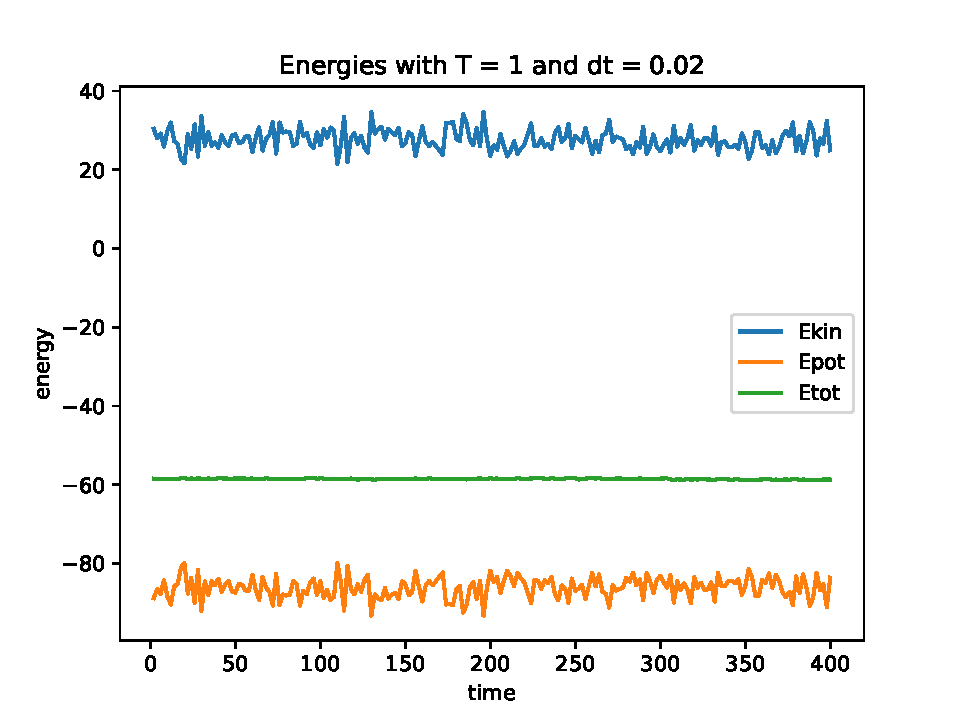
\includegraphics[width=\textwidth]{img/3_2a_dt002.pdf}
  \end{minipage}
\end{figure}

\begin{figure}[!ht]
  \centering
  \begin{minipage}{0.49\textwidth}
    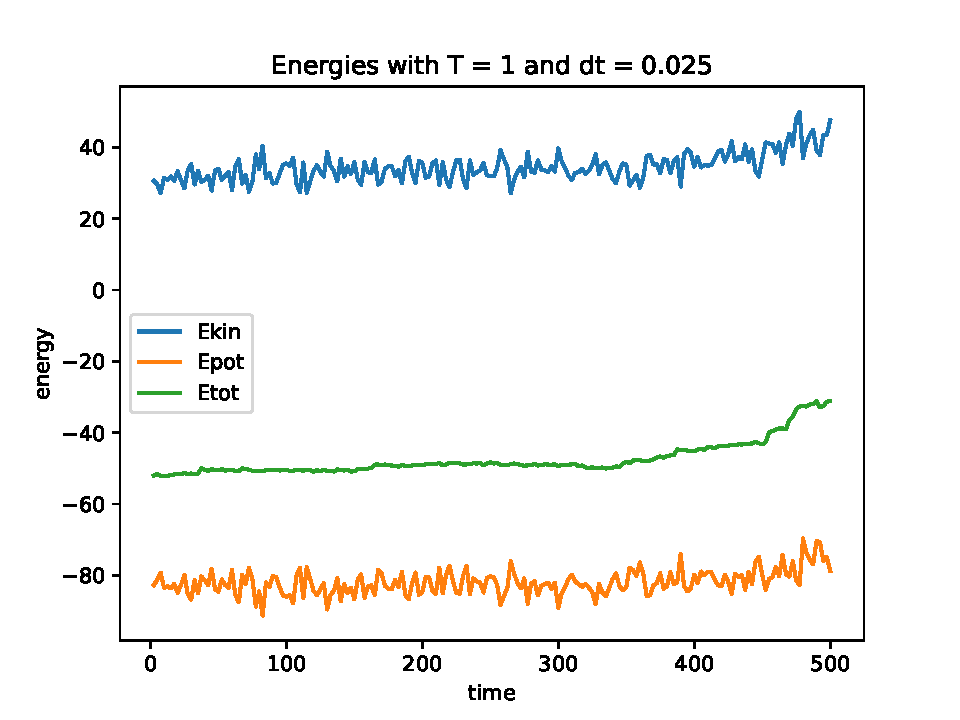
\includegraphics[width=\textwidth]{img/3_2a_dt0025.pdf}
  \end{minipage}
  \begin{minipage}{0.49\textwidth}
    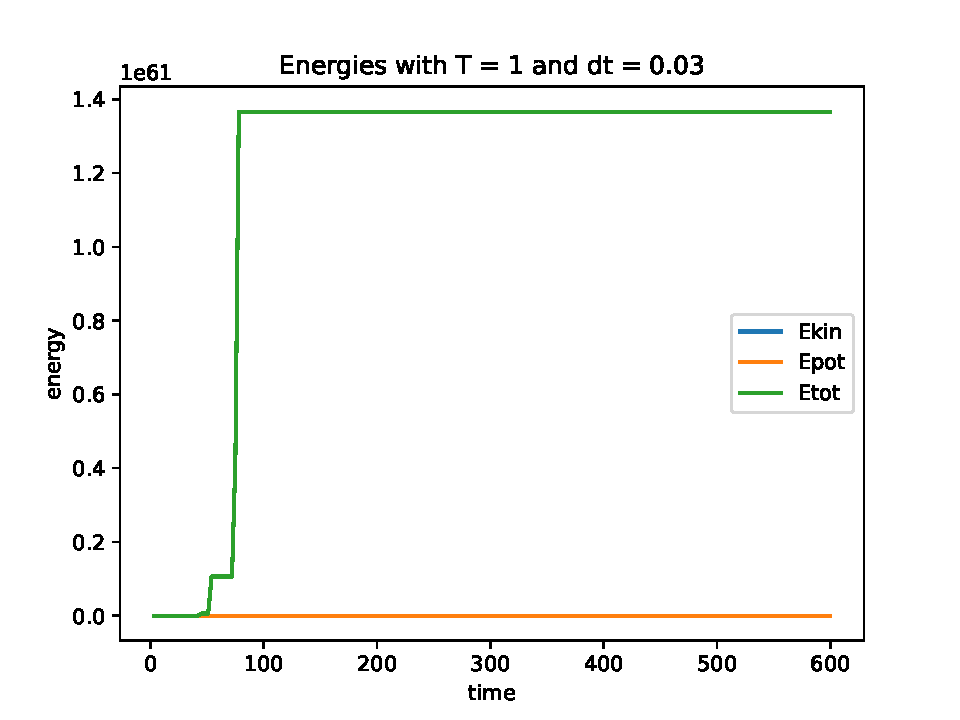
\includegraphics[width=\textwidth]{img/3_2a_dt003.pdf}
  \end{minipage}
\end{figure}

\FloatBarrier

Do note that the time axes aren't identical, due to how the template code calculates the running time. Using
\texttt{dt} $= 0.01$ leads to the total energy being conserved well, since the green line doesn't fluctuate at all.
The same is almost true for \texttt{dt} $= 0.02$, however here one can start to notice some "imperfections", as the
line isn't \emph{perfectly} smooth anymore. Increasing the time step to $0.025$, the quality of integration is really
poor, since the energy now drifts considerably. In some cases we already start seeing havoc here, but setting the time
step to $0.03$ ensures this behavior. Now the kinetic energy of the system has been severely miscalculated, making the
simulation useless. In all remaining parts of this exercise, a timestep of $0.01$ has been used (unless explicitly
stated otherwise) to ensure the quality of integration remains good.

\subsection*{Part b}

Running a LJ simulation using $T = 0.2$ gives the following result:

\begin{figure}[!ht]
  \centering
  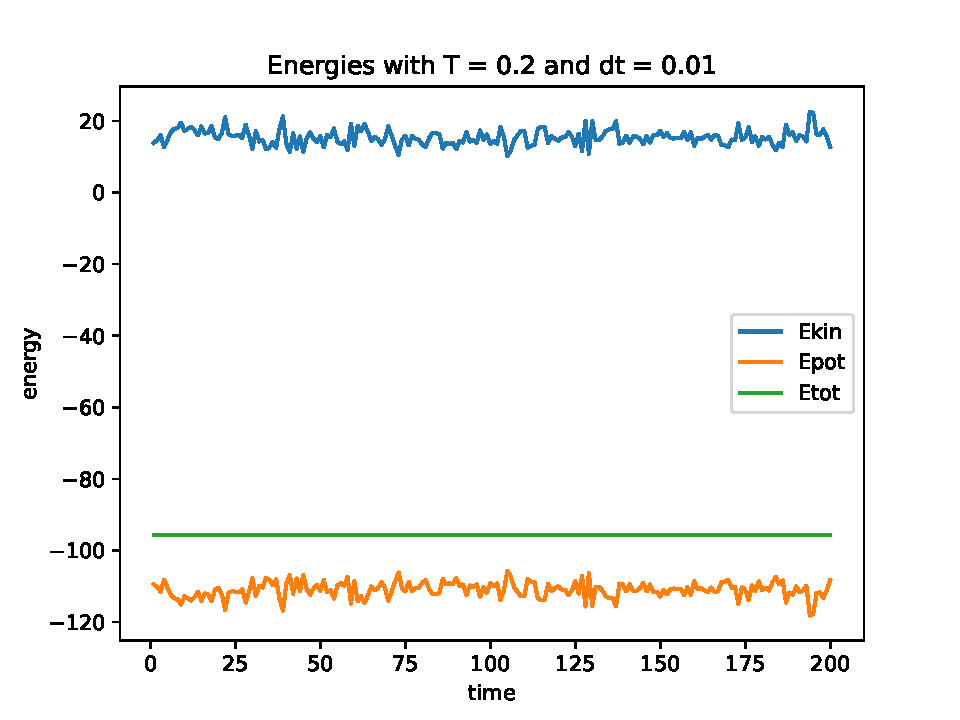
\includegraphics[scale=0.49]{img/3_2b.pdf}
\end{figure}

Compared to $T = 1$, we observe lower energies (speaking in terms of the magnitude) in the system overall, as well as
the fluctuations being slightly smaller.

\subsection*{Part c}

Implementing an Andersen thermostat that thermalizes all particles simulaneously at a fixed step interval $n$ (in this
case $10$, since that was the given parameter in the code) and running simulations at $T = 1$ and $0.2$ yields:

\begin{figure}[!ht]
  \centering
  \begin{minipage}{0.49\textwidth}
    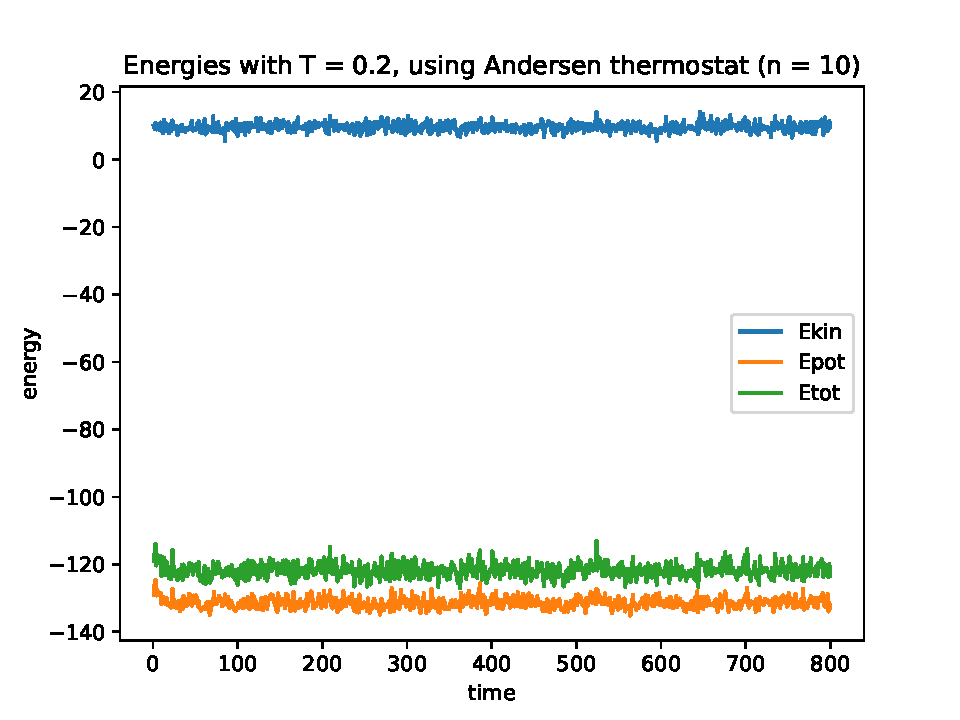
\includegraphics[width=\textwidth]{img/3_2c_T02_n10.pdf}
  \end{minipage}
  \begin{minipage}{0.49\textwidth}
    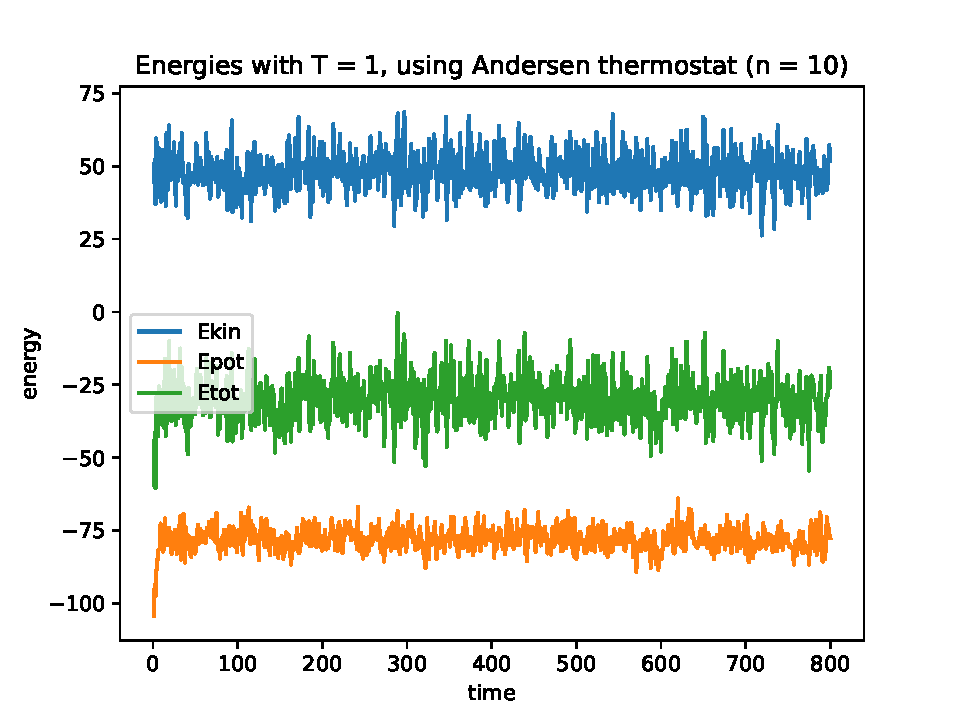
\includegraphics[width=\textwidth]{img/3_2c_T1_n10.pdf}
  \end{minipage}
\end{figure}

Comparing the graphs to their non-thermostat versions, a couple of things are immediately apparent:

\begin{itemize}
  \item The total energy now fluctuates, as a consequence of how the Andersen thermostat is designed.
  \item The potential energies seem to converge to a value different from what they started on.
  \item A higher temperature implies the fluctuations magnitude to be bigger, especially in regards to the kinetic
        energy.
\end{itemize}

To answer the physics question of if we can explain what we see, the last point is especially important. Looking at
the graphs as well as the animations for each temperature of the system, it can be reasonable to conclude that we're
looking at some sort of liquid when $T = 0.2$ and a gas when $T = 1$, since some chaotic behavior can be spotted at
higher temperatures.

\subsection*{Part d}

Judging from Part c of this exercise, the energies in the system seems to converge quickly to their final value. But
in order to truly be safe, only the energies in the last $80\%$ of the simulation was used in the calculations to
estimate the average. To estimate the heat capacity, the last value generated was used since there weren't really any
oscillatins or fluctuations to observe in that parameter. Running the simulation with the Andersen thermostat for
different temperatures yields the following plot:

\begin{figure}[!ht]
  \centering
  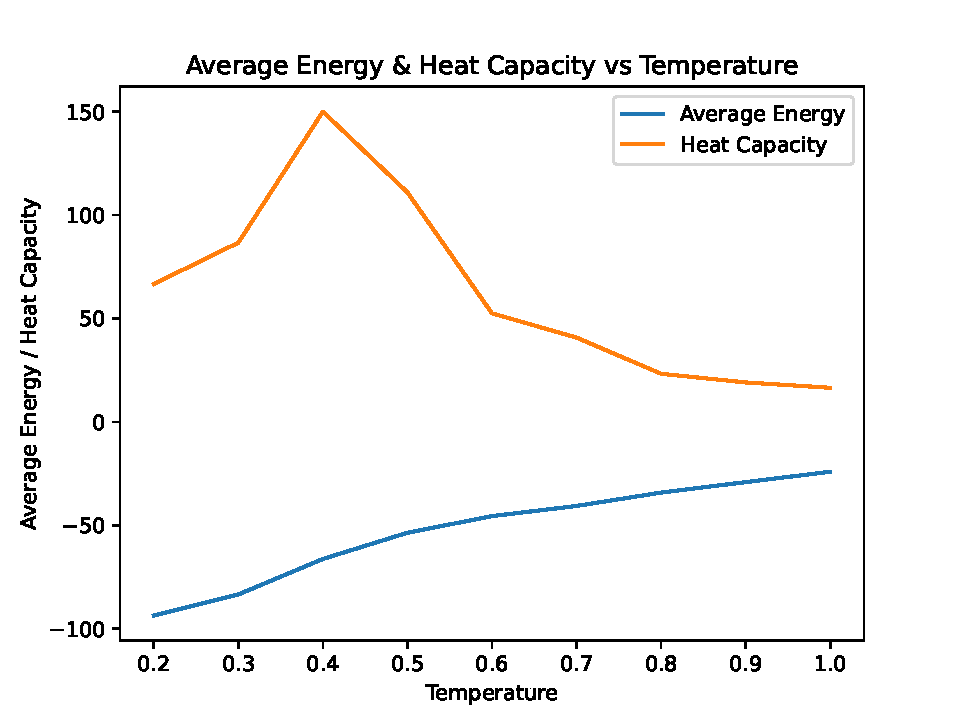
\includegraphics[scale=0.49]{img/3_2d_ECvvsT.pdf}
\end{figure}

\FloatBarrier

The total energy in the system slowly increases as we raise the temperature, which in turn also leads to more chaotic
motion of the particles. The heat capacity decreases as the temperature is raised, but what's interesting to note is
that the local maxima doesn't appear at one of the end points.

\subsection*{Part e}

Now we turn our attention to the pressure $p$ of the system. Pressure can be related to volume and temperature by the
ideal gas law:

$$
  pV = Nk_BT = nRT
$$

Where $N$ is the number of particles, $k_B$ the Boltzmann constant, and $T$ the temperature. The law may also be
stated in terms of the amount of substance $n$ of the system as well as the universal gas constant $R$, but for our
purposes in doing a simulation where the exact number of particles is easily known, the former representation is the
one to prefer. Running the simulation for different temperatures and also for a unit cell that's 4x the size (by
doubling L), extracting the final pressure after the simulation has run and plotting it, as well as plotting the 
pressure calculated through the ideal gas law yielded the following:

\begin{figure}[!ht]
  \centering
  \begin{minipage}{0.49\textwidth}
    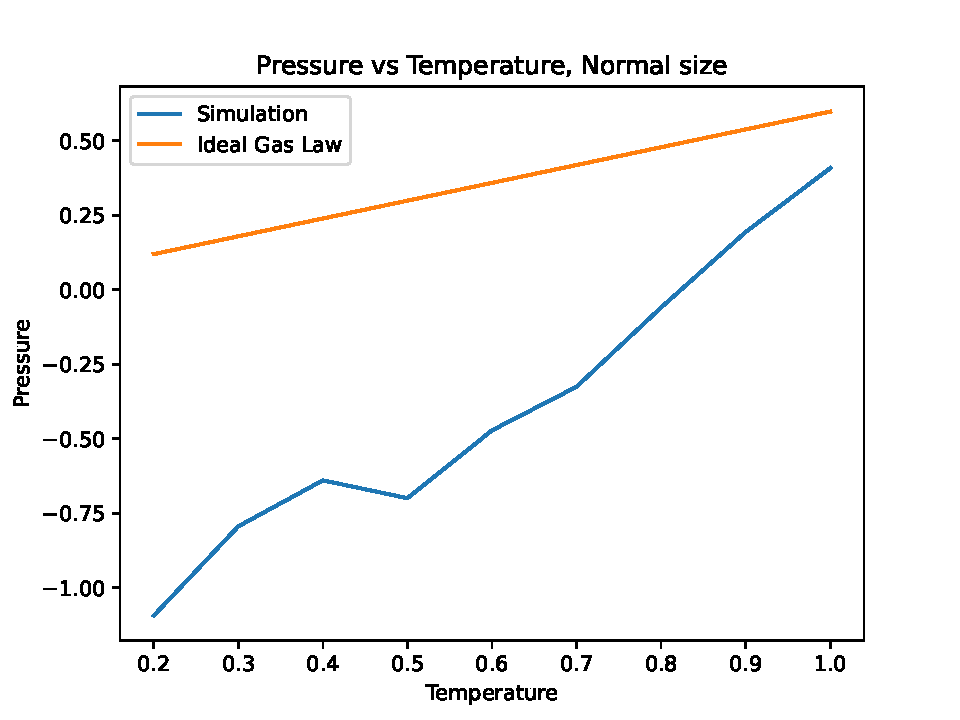
\includegraphics[width=\textwidth]{img/3_2e_PvsT_normal.pdf}
  \end{minipage}
  \begin{minipage}{0.49\textwidth}
    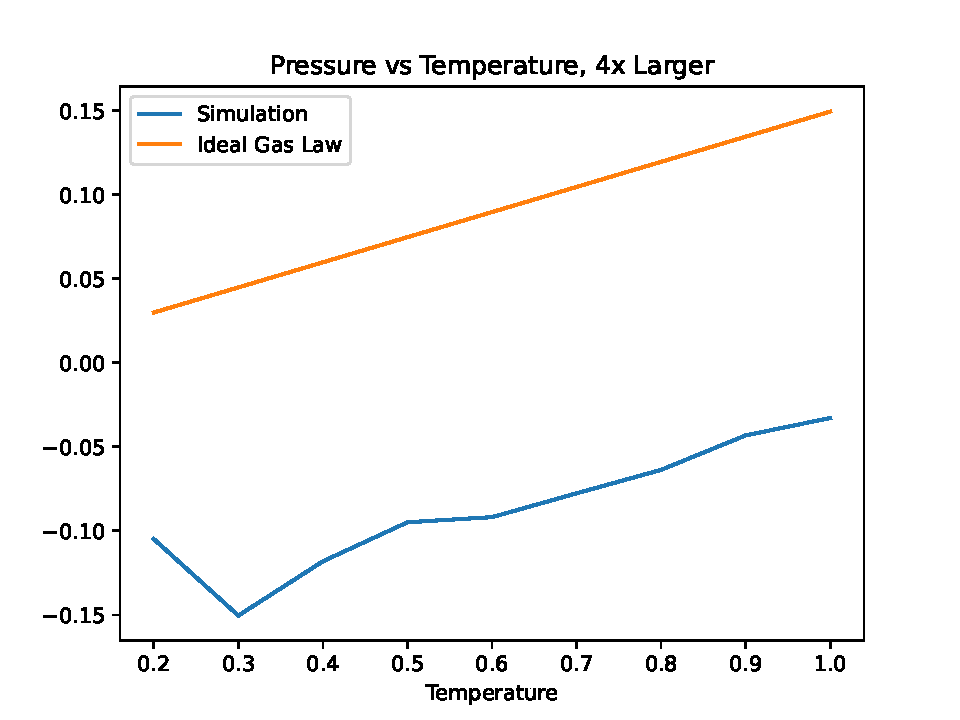
\includegraphics[width=\textwidth]{img/3_2e_PvsT_big.pdf}
  \end{minipage}
\end{figure}

As might be expected, the pressure increases when the temperature is raised. Though for the smaller of the two
systems, the rate at which it increases isn't tied to the ideal gas law. Compare that to the second system, where the
rate at which it increases more closely resembles the slope of the ideal gas law. As to why the lines don't overlap,
keep in mind that this is a simulation of a finite number of particles interacting, while the ideal gas law doesn't
take boundary conditions or the number of molecules into consideration, since that does end up affecting the result.

\end{document}